\chapter{Problem Background}
\label{ch:problem_background}
Jointly the thesis I was willing to develop a neural net model for automatic spine vertebrae segmentation of computer tomography scans (images). CT is a preferred image modality to examine the bone part of a spine due to high bone-to-soft-tissue contrast. As I learned, before proceeding with analysing the bones themselves we need to precisely reconstruct and label our data. Owing to \href{https://biomedia.doc.ic.ac.uk/}{\color{blue}"BioMediaA"} laboratory I was capable to use already collected and labeled dataset.             



Image segmentation \cite{Shapiro2001} is the process of partitioning a digital image into multiple segments (sets of pixels, also known as image objects). The goal of segmentation is to simplify and/or change the representation of an image into something that is more meaningful and easier to analyze. In mathematical terms, the aim is to find a closed contour $\Gamma$ that partitions a domain $\Omega \in \mathbb{R}$  into subregions $\Omega_i, i = 1, 2, ..., N$.
The very first notation was established by David Mumford $\footnote{ \url{https://en.wikipedia.org/wiki/David_Mumford}}$ in 1989 and obtained name \cite{Kim2020} Mumford-Shah functional.

\section{Mumford-Shah functional}
Mumford-Shah functional considers the piecewise smooth approximation of an input image $z(x)$ by a pair $(\upsilon, \Gamma)$. Assume $\Omega$ be a bounded domain in $\mathbb{R}$ and $z(x)$ be a bounded measurable function defined on $\Omega$. The functional is defined as follows:
\begin{align*}
 E (\upsilon, \Gamma) = \upsilon H^{n-2} (\Gamma) + \mu^2 \int_{\Omega} (\upsilon - z)^2 \partial x + \int_{\frac{\Omega}{\Gamma}} \lvert \nabla \upsilon \rvert^2 \partial x
 \end{align*}

The functional contains a fidelity term on $\upsilon \in \complement^1$ and two regularity terms. One
imposes smoothness on $\upsilon$ and the others imposes regularity on $\Gamma$ in terms of its one dimensional \cite{Buda1992} Hausdorff measure.

Mumford and Shah also introduced the restriction of $E$ to piecewise-constant functions $\upsilon$. In other words $\upsilon = c_k$ on each open set $\Omega_k$, where $c_k$ stands for average value of $z$ in each region $\Omega_k$. The piecewise-constant Mumford-Shah functional is defined as:

\begin{align*}
 E_0 (\upsilon, \Gamma) = \upsilon H^{n-1} (\Gamma) \int_{\Omega_k} (\upsilon - c_k)^2 \partial x
\end{align*}

It can be proved that $E_0$ is the natural limit functional of $E$ as $\mu \to 0$. This is linked, in the discrete setting, to the \cite{Wu1982} Potts Model which has been widely studied. The above functional is the basis for a significant amount of important work in field of image segmentation.

\section{Data description}
%TODO change
The data set consists of spine-focused CT scans of 125 patients with varying types of pathologies. 

In the case of the detection model the dense labelling contains two values: 0 representing background and 1 representing vertebrae. 

The identification model’s dense labelling contains values from 0 to 26. Whilst 0 representing background, 1 representing C1 vertebrae up to 26 representing S2 vertebrae.

\begin{figure}[h]
    \centering 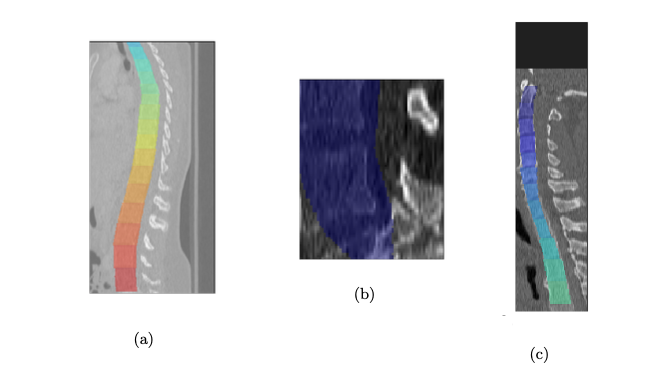
\includegraphics[width=9cm]{images/labeled_data.png}
    \caption {(a) shows a dense labelling, (b) shows an example of a sample used to train the detection model, (c) shows an example of a sample used to train the identification model. Note: The size of the sample is 8 x 80 x 320, if the original scan is not larger enough to fill those dimensions some padding is added, as can be seen at the top.}
    \label{fig:labeled_data}
\end{figure}
